%%%%%%%%%%%%%%%%%%%%%%%%%%%%%%%%%%%%%%%%%%%%%%%%%%
%%%%		~~~~ HPM ~~~~
%%%%%%%%%%%%%%%%%%%%%%%%%%%%%%%%%%%%%%%%%%%%%%%%%%


\chapter{La méthode de Perturbation d'Homotopie}
\label{chap:RN_EDF}
\pagestyle{fancy}

\section{Introduction}
Les équations différentielles fractionnaires occupent une place particulière en raison de leur complexité et de leurs application à divers domaines scientifiques et techniques. Cependant, elle admet rarement des solutions explicites exprimées à l'aide de fonctions usuelle.
Il existe plusieurs méthodes numériques pour résoudre ces équations comme la méthode d'itération variationnelle, la méthode d'Euler, la méthode d'Adams, la méthode de différence finie et la méthode de perturbation d'homotopie.

Dans ce chapitre nous allons appliquer la méthode de perturbation d'homotopie pour résoudre des équations différentielles fractionnaires au sens de Caputo. Cette méthode est une technique semi-analytique puissante, née de la combinaison de deux concepts: la technique de perturbation, qui manipule l'équation pour faciliter la résolution, et la technique d'homotopie, qui établie un chemin continue entre deux solutions d'une équation \cite{Advanced_Numerical}.

Historiquement, la MPH a été proposé et développée pour la première fois par le Professeur Ji-Huan He dans les années 1990. Elle était sa réponse innovant aux limites des méthodes traditionnelles, souvent entravées par l'existence d'un petit paramètre \cite{HPM_original}.

Cette méthode est fondamentalement une approche flexible pour résoudre divers types d'équations différentielles, notamment les équations différentielles non linéaires, les équations différentielles à dérivées partielles et les équations différentielles fractionnaires. 

L'intuition de la méthode HPM est la transformation d'une équation difficile à résoudre en une série d'équations plus faciles, en construisant une équation d'homotopie qui fournit une approximation continue de la solution exacte \cite{Advanced_Numerical}. L'une des plus grandes forces cet méthode réside dans sa capacité à fournir des solutions approchées sous forme de séries convergentes rapidement, même pour les problèmes difficiles.

\section{Application de la méthode aux équations différentielles ordinaires}
La méthode de perturbation homotopique repose sur des principes mathématiques fondamentaux qui s'appliquent aux équations différentielles ordinaires. Ces principes peuvent ne pas être immédiatement transférables aux équations fractionnaires, qui possèdent des propriétés et des complexités supplémentaires. En testant d'abord la méthode sur les équations différentielles ordinaires, nous pouvons comprendre et maîtriser le fonctionnement de la méthode, et nous assurer qu'elle est solide et précise. 
\subsection{Description de la méthode}
Soient X et Y deux espaces topologiques. On dit que deux applicationss continues $f,g:X\mapsto Y$ sont homotopiques s'il existe une application continue :
\begin{align*}
    F:X \times [0,1] & \mapsto Y \\
    (x,p) &\mapsto F(x,p)
\end{align*}
telle que:
\begin{equation*}
    F(x,0)=f(x)
\end{equation*}
et
\begin{equation*}
    F(x,1) = g(x)
\end{equation*}
Pour mieux illustrer l'idée de base de ce cette méthode, nous allons considérer l'équation différentielle non linéaire suivante:
\begin{equation} \label{eq:def_ED}
    A(u)-f=0, \hspace{1cm} r\in\Omega
\end{equation}
avec les conditions aux limites:
\begin{equation}
    B(u,\frac{\partial u}{\partial n}) = 0, \hspace{1cm} r\in \Gamma
\end{equation}
où $A$ est un opérateur différentiel général, $B$ opérateur limit, $f$ est une fonction connue et $\Gamma$ est la frontière de $\Omega$.\\
En général, l'opérateur $A$ peut être écrit sous la forme $A=L+N$, où $L $ désigne un opérateur linéaire et $N$ un opérateur non linéaire, alors l'équation \ref{eq:def_ED} devient: 
\begin{equation}
    L(u) + N(u) - f =0
\end{equation}
Construisons maintenant une homotopie $v(r,p): \Omega \times[0,1] \mapsto \mathbb{R}$, qui satisfait:
\begin{equation}\label{eq:sol_hom1}
    H(v,p)=(1-p)[L(v)-L(u_0)]+p[A(v)-f]=0, \hspace{1cm} p\in [0,1],
\end{equation}
où
\begin{equation}\label{eq:sol_hom2}
    H(v,p) = L(v)-L(u_0) +pL(u_0)+p[N(v)-f]=0,
\end{equation}
avec $p\in[0,1]$ est un paramètre d'homotopie, $u_0$ est une approximation initiale de la solution de l'équation \ref{eq:def_ED} satisfaisant les conditions aux limites. Les formules \ref{eq:sol_hom1} et \ref{eq:sol_hom2} impliquent:
\begin{equation}
    H(v,0)=L(v)-L(u_0)=0,
\end{equation}
\begin{equation}
    H(v,1)=A(v)-f=0,
\end{equation}
$u_0$ se transforme en $u$ grâce au changement du paramètre $p$ de zéro à 1. En topologie, avec cette propriété la fonction $v$ est appelé une homotopie. Maintenant, supposons que la solution de \ref{eq:sol_hom1} et \ref{eq:sol_hom2} sont exprimées comme:
\begin{equation}
    v=v_0+pv_1+p^2v_2+p^3v_3+ .... = \sum_{i=0}^{\infty}v_ip^i
\end{equation}
La solution analytique approché de l'équation \ref{eq:def_ED} est donnée par :
\begin{equation}
    u=\lim_{p\mapsto1}v = v_0 + v_1+v_2 +...
\end{equation} 
\subsection{Application}
\subsubsection*{Exemple 1}
Considérons l'équation différentielle non linéaire suivante:
\begin{equation} \label{ex:EDO_1}
    \begin{cases}
        u'(t)+u^2(t)=0, \hspace{1cm} t\geq 0,\\
        u(0)=1,
    \end{cases}
\end{equation}
où la solution exact est donnée par:
\begin{equation}
    u(t)=\frac{1}{1+t}.
\end{equation}
Selon la méthode de la perturbation d'Homotopie, nous pouvons construire l'homotopie suivante :
\begin{equation*}
    H: \Omega\times[0,1] \mapsto\mathbb{R}
\end{equation*}
\begin{align}
    (1-p)\left(v'(t)-u'_0(t)\right)+p\left(v'(t)+v^2 (t))\right), \hspace{0.5cm} p\in[0,1], \hspace{0.5cm} t\in \Omega
\end{align}
avec $u_0=u(0)=1$.\\
La solution de l'équation \ref{ex:EDO_1} peut être exprimée comme suit:
\begin{equation}\label{sol:EDO_1}
    v=v_0+pv_1+p^2v_2+p^3v_3...=\sum_{k=0}^{\infty} p^{k}v_k.
\end{equation}
Substituons l'équation \ref{sol:EDO_1} dans l'équation \ref{ex:EDO_1} et identifions les termes de même puissance de $p$, il vient:
\begin{align*}
    \begin{cases}
        &p^0 : v'_0(t) = u'_0(t),\\
        &p^1 : v'_1(t) = u'_0(t)-v^2_0(t), \hspace{1cm} v_1(0)=0,\\
        &p^2 : v'_2(t) = -2v_0(t)v_1(t), \hspace{1cm} v_2(t)=0,\\
        &    .\\
        &    .\\
        &    .\\
    \end{cases}
\end{align*}
Par conséquent, nous obtenons:
\begin{align*}
    &v_0(t)=1,\\
    &v_1(t)=-t,\\
    &v_2(t)=t^2.
\end{align*}
Finalement, la solution approchée de l'équation \ref{ex:EDO_1} est donnée par :
\begin{equation}
    u(t)=\lim_{p \to 1} v(t) = v_0(t)+v_1(t)+v_2(t) + ... = 1-t + t^2 ...
\end{equation}
\begin{figure}[H]
    \centering
    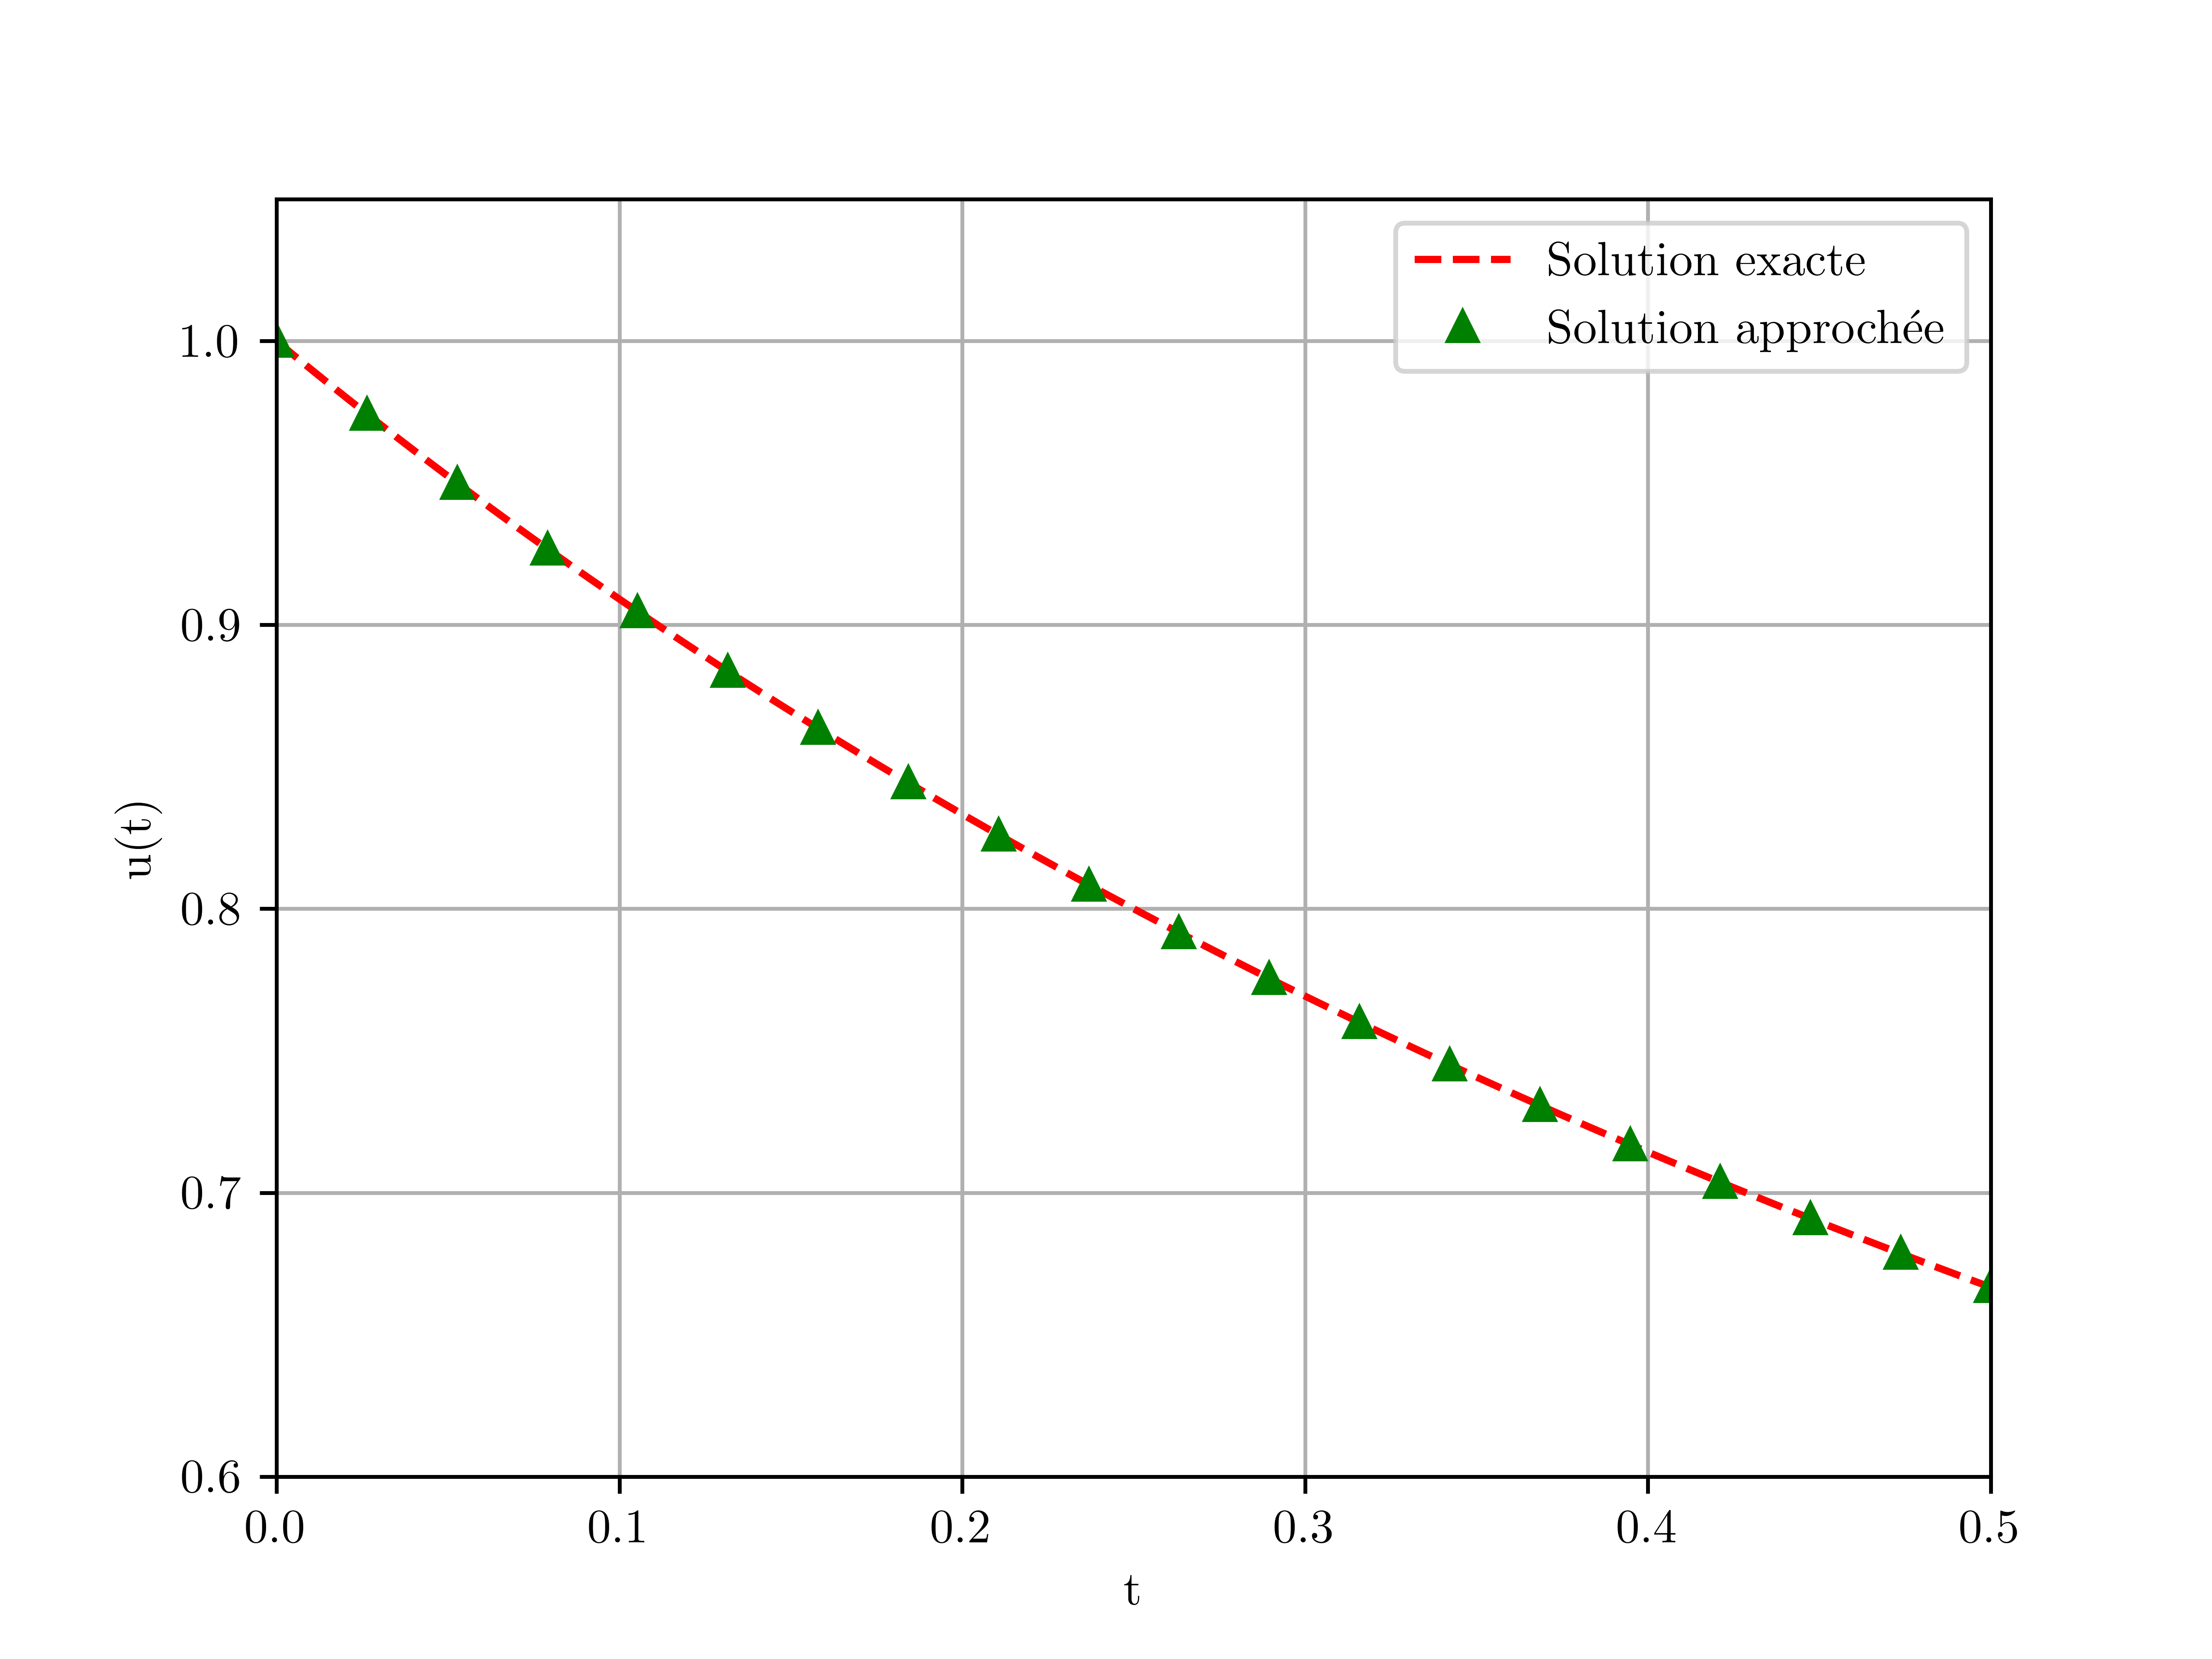
\includegraphics[scale = 0.7]{IMAGES/plot.png}
    \caption{Comparaison entre la solution exacte et la solution approchée en utilisant la MPH.}
    \label{fig:sol_EDO_1}
\end{figure}
\subsubsection*{Exemple 2}
Maintenant, nous allons considérer l'équation de Lane-Emden suivante:
\begin{equation}\label{ex:EDO_2}
    \begin{cases}
        u''(x)+\frac{2}{x}u'(x)+u(x) = x^5 + 30x^3,\\
        u(0) = u'(0)=0,
    \end{cases}
\end{equation}
où la solution exacte est exprimée par:
\begin{equation}
    u(x)=x^5.
\end{equation}
La méthode de perturbation d'Homotopie, implique :
\begin{equation} \label{sol:EDO_2}
    \left(v''+\frac{2}{x}v'\right) - \left(u''_0+\frac{2}{x}u'_0 \right) = p\left(x^5+30x^3-v-u''_0 - \frac{2}{x}u'_0\right).
\end{equation}
La solution de l'équation \ref{ex:EDO_2} est sous la forme:
\begin{equation}
    v=v_0+pv_1+p^2v_2+p^3v_3 + ...
\end{equation}
Substituons l'équation \ref{sol:EDO_2} dans l'équation \ref{ex:EDO_2} et identifions les termes de même puissance de $p$, il vient :\\
\begin{align*}
    \begin{cases}
        &p^0 : v_0(x) = u_0(x)=0,\\
        &p^1 : v_1(x)=\frac{1}{56}x^7 + x^5,\\
        &p^2 : v_2(x) = -\frac{1}{5040}x^9 - \frac{1}{56}x^7,\\
        &p^3 : v_3(x) = \frac{1}{665280}x^{11}+\frac{1}{5040}x^9,\\
        &p^4 : v_4(x) = \frac{1}{121080960} x^{13} - \frac{1}{665280}x^{11},\\
        &p^5 : v_5(t) = \frac{1}{29059430400}x^{15} + \frac{1}{121080960} x^{13},\\
        &    .\\
        &    .\\
        &    .\\
    \end{cases}
\end{align*}
Finalement, la solution approchée le d'équation \ref{ex:EDO_2} est donnée par:
\begin{equation}
    u(x)=\lim_{p\to 1} v(x)=v_0(x)+v_1(x)+v_2(x)+...
\end{equation}
\begin{figure}[H]
    \centering
    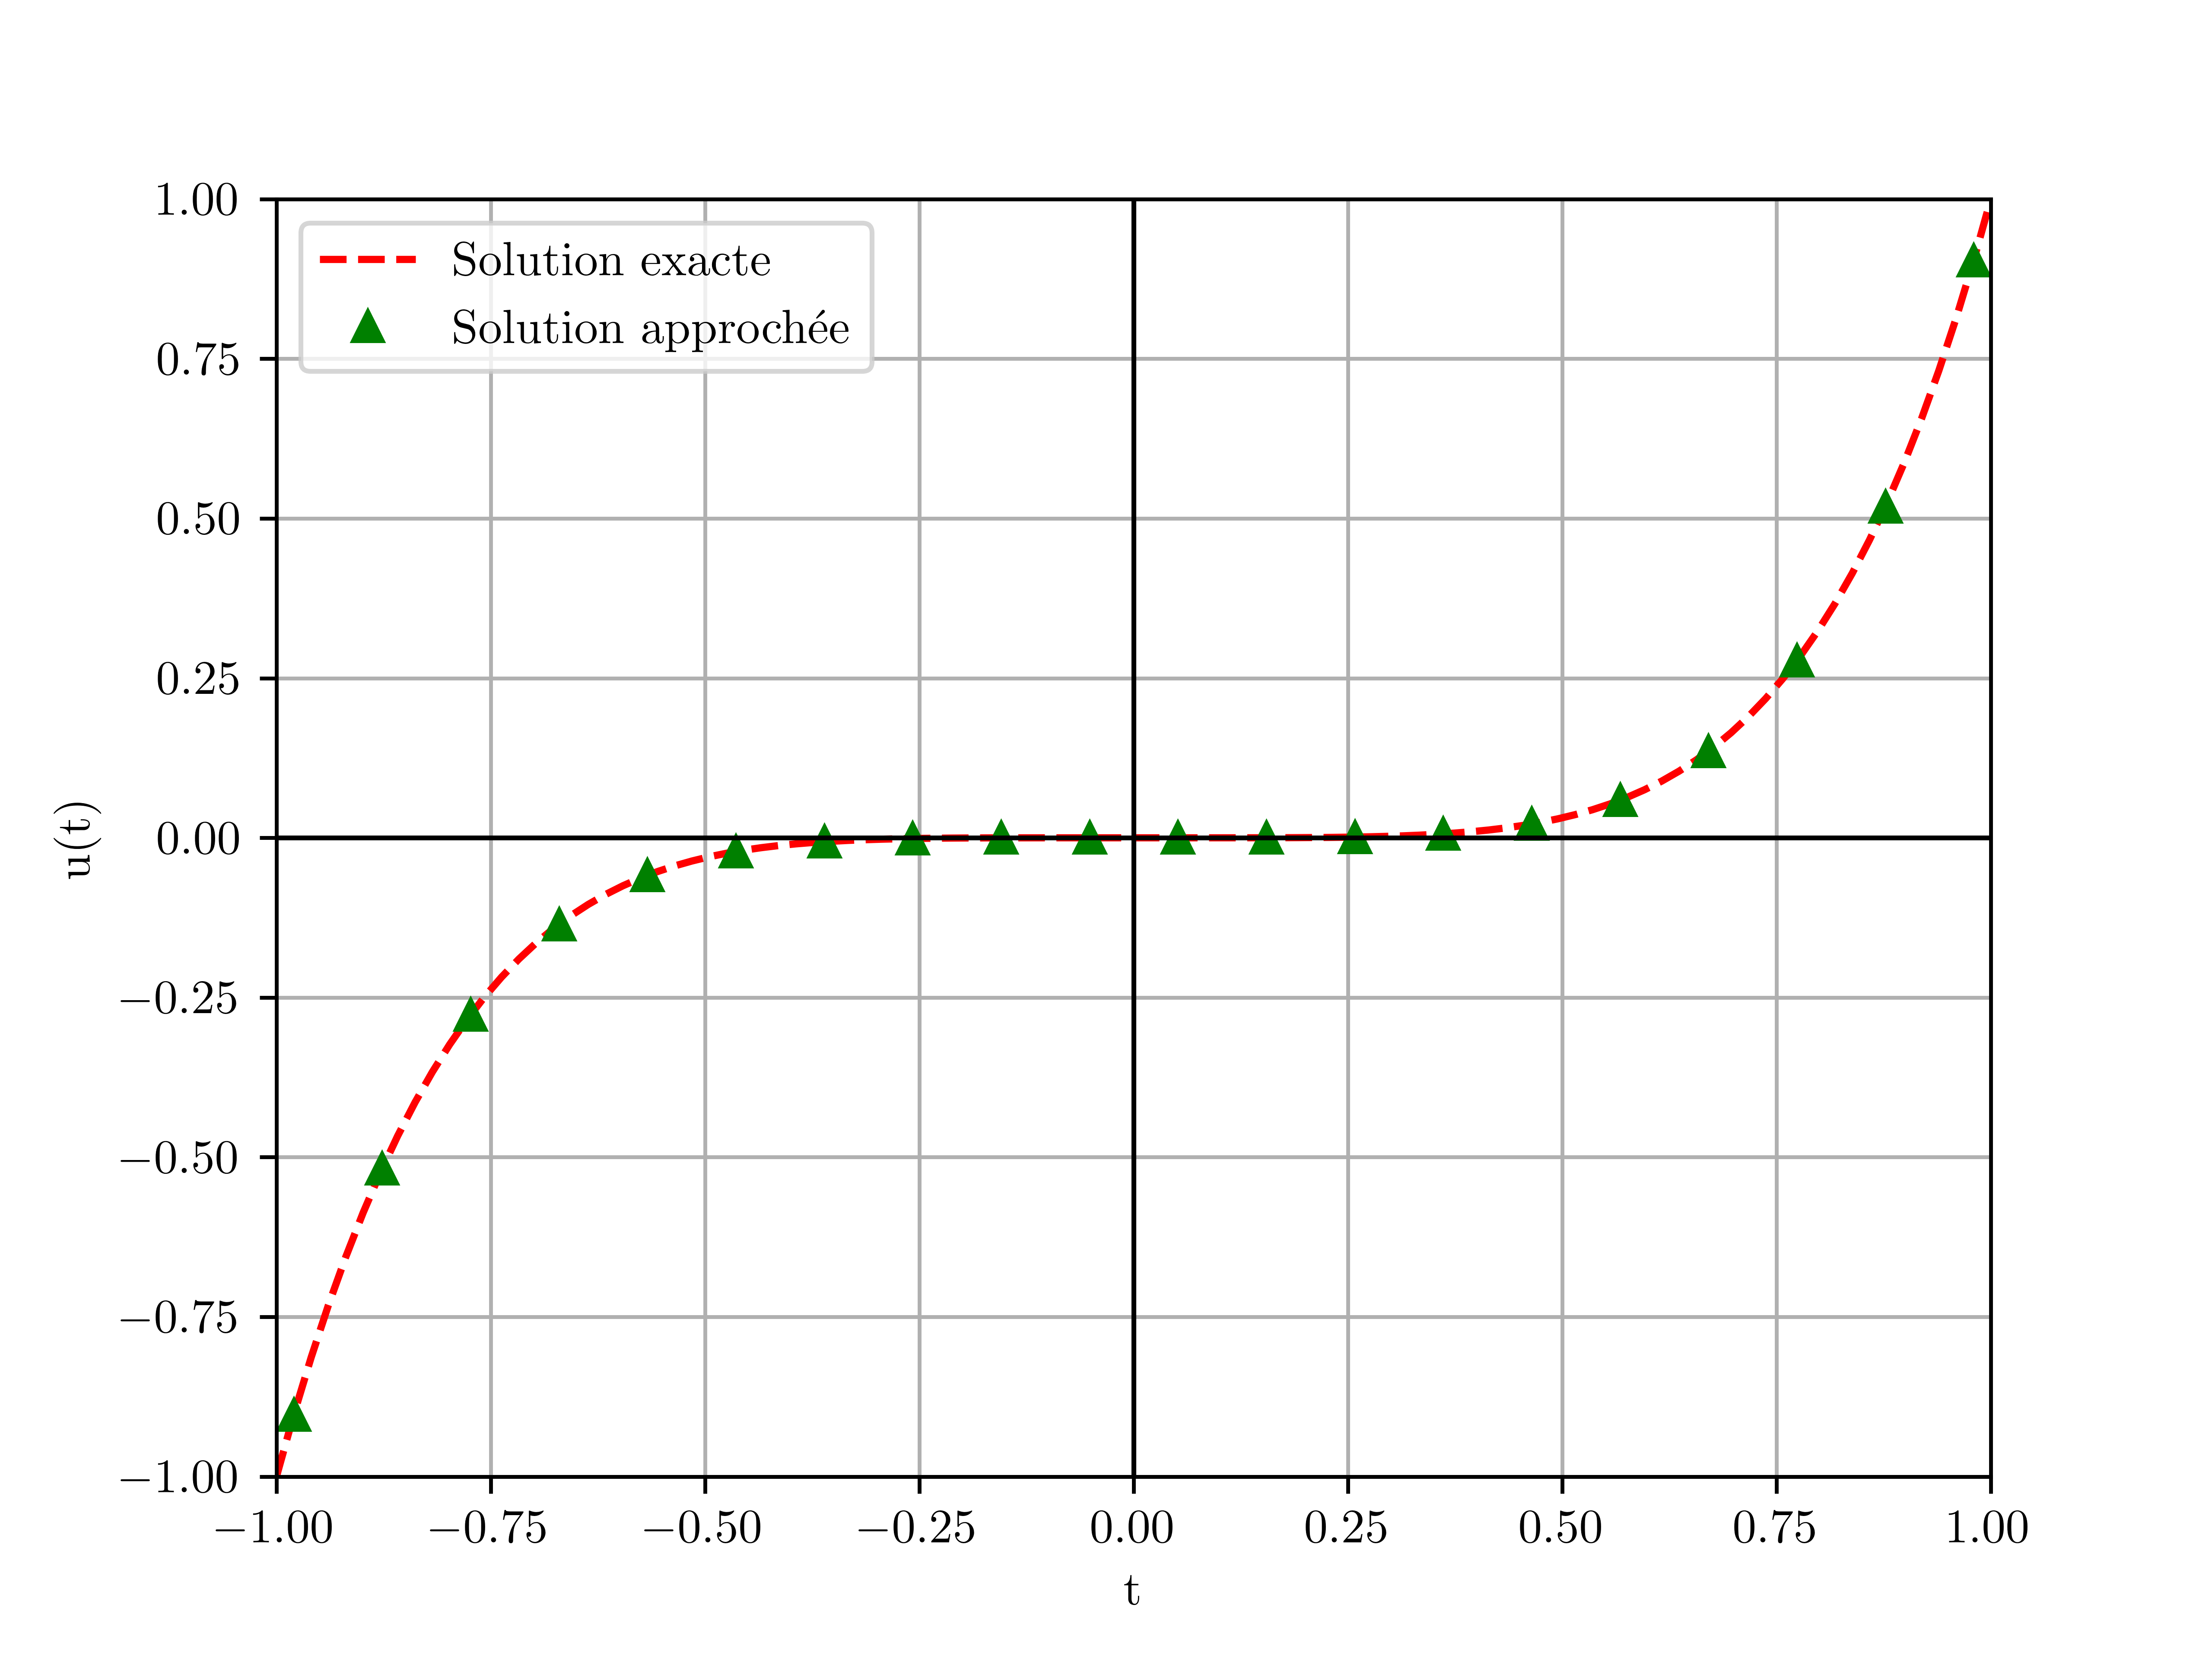
\includegraphics[scale = 0.7]{IMAGES/plot (2).png}
    \caption{Comparaison entre la solution exacte et la solution approchée en utilisant la MPH.}
\end{figure}



\section{Application de la méthode aux équations différentielles fractionnaires}
\subsection{Description de la méthode}
 Le problème de valeur initiale d'équations différentielles fractionnaires est donnée par sa forme opérationnelle:
 \begin{align}\label{eq: HMP_EDF_theorie}
     D^{\alpha} f(t) + Lf(t) = g(t)\\
     f^{(i)} (0) = c_i, \hspace{1cm} i=0,1,2, ..., n-1
 \end{align}
 où $c_i$ est la condition initial, $L$ désigne un opérateur linéaire qui peut inclus d'autre opérateurs de dérivées fractionnaires $D^{\beta}(\beta < \alpha)$ et $g$ est une fonction connue.
\\
L'homotopie de l'équation \ref{eq: HMP_EDF_theorie} satisfait :
  \begin{equation}\label{eq:HPM_FDE_1}
      (1-p)D^{\alpha} f +p\left[ D^{\alpha}f + Lf(t) -g(t)\right]=0, \hspace{1cm} p\in [0,1],
  \end{equation}
  où
  \begin{equation}\label{eq:HPM_FDE_2}
      D^{\alpha}f+p\left[Lf(t)-g(t)\right]=0,
  \end{equation}
  avec $p\in[0,1]$ est un paramètre d'homotopie. Si $p=0$, l'équation \ref{eq:HPM_FDE_1} et \ref{eq:HPM_FDE_2} devient:
  \begin{equation}
      D^{\alpha} f=0
  \end{equation}
  Si $p=1$, les deux équations \ref{eq:HPM_FDE_1} et \ref{eq:HPM_FDE_2} donnent l'EDF original \ref{eq: HMP_EDF_theorie}.\\
  La solution de l'équation \ref{eq: HMP_EDF_theorie} est:
  \begin{equation} \label{eq:sol_HPM_theorie}
      f(t)=f_0(t)+pf_1(t)+p^2f_2(t)+p^3f_3(t) + ...
  \end{equation}
  Substituons l'équation \ref{eq:sol_HPM_theorie} dans l'équation \ref{eq:HPM_FDE_2} et identifions les termes de même puissance de $p$, il vient:
  \begin{align*}
  \begin{cases}
            & p^0 : D^{\alpha} f_0 = 0\\
      & p^1 : D^{\alpha} f_1 = -Lf_0 + g(t)\\
      & p^2 : D^{\alpha} f_2 = -Lf_1(t)\\
      & p^3 : D^{\alpha} f_3 = -Lf_2(t)\\
      & .\\
      & .\\
  \end{cases}
  \end{align*}
on peut réécrit les termes de solution de perturbation d'homotopie par :
\begin{align*}
    \begin{cases}
        & f_0 = \sum_{i=O}^{m-1} f^{(i)}(0) \frac{t^i}{i!} = \sum _{i=0}^{m-1} c_i \frac{t^i}{i!} \\
          & f_1 = -I^{\alpha} [Lf_0(t)] + I^{\alpha}[Lg(t)]\\
          & f_2 = -I^{\alpha}[Lf_1(t)]\\
          & f_3 = -I^{\alpha}[Lf_2(t)]\\
          & .\\
          & .\\
    \end{cases}
  \end{align*}
La forme générale de la solution HPM est donné par :
\begin{equation}
    f_n=-I^{\alpha}[Lf_{n-1}(t)]
\end{equation}
Alors la solution de perturbation d'homotopie est :
\begin{equation}
    f(t)=f_0+f_1+f_2+f_3 + ... +f_n + ...
\end{equation}
\subsection{Application}
\subsubsection*{Exemple 1}
Considérons l'équation différentielle fractionnaire linéaire suivante:
\begin{equation}
    \begin{cases}\label{ex:EDF_1}
        D^{\alpha}x(t) + x(t) = \frac{2}{\Gamma(3-\alpha)} t^{2-\alpha} + t^3,\\
        x(0)=0,\\
        x'(0)=0.
    \end{cases}
\end{equation}
où la solution exacte pour $\alpha = 1,9$ est donnée par:
\begin{equation}
    x(t)=t^2.
\end{equation}
Selon la méthode de perturbation d'Homotopie, nous pouvons construire l'homotopie suivante:
\begin{equation} \label{eq:HPM_EDF1}
    D^{\alpha} x(t) +p\left[x(t)-\frac{2}{\Gamma(3-\alpha)}t^{2-\alpha}-t^3\right] =0, \hspace{1cm} t\in \Omega,
\end{equation}
La solution de \ref{ex:EDF_1} peut être exprimée comme suit :
\begin{equation}\label{sol:EDF_1}
    x(t) =x_0(t) + px_1(t) + p^2x_2(t) + ... = \sum _{i=O}^{\infty} p^i x_i(t)
\end{equation}
Substituons l'équation \ref{sol:EDF_1} dans l'équation \ref{eq:HPM_EDF1} et identifions les termes de même puissance de $p$, il vient :
\begin{align*}
    \sum_{i=0}^{\infty} D^{\alpha} p^{(i)} x_i(t) = -p\left[\sum_{i=0}^{\infty} p^{(i)} x_i(t) -\frac{2}{\Gamma(3-\alpha)} t^{2-\alpha} -t^3\right]
\end{align*}
\begin{align} \label{eq:p_1}
    \begin{cases}
    & p^0 : D^{\alpha}x_0(t)=0, \\
    & p^1 : D^{\alpha}x_1(t) = -x_0(t) + \frac{2}{\Gamma(3-\alpha)} t^{2-\alpha} + t^3,\\
    & p^2 : D^{\alpha} x_2(t) = -x_1(t),\\
    & p^3 : D^{\alpha} x_3(t) = -x_2(t),\\
    &     . \\
    &     .\\
    &     .\\
    \end{cases}
\end{align}
Appliquent l'opérateur $I^{\alpha}$ sur les deux cotés de d'équations \ref{eq:p_1} et on utilisons les propriétés de L'intégrale fractionnaire de Riemann-Liouville d'ordre $\alpha \geq 0$, on obtient 
\begin{align*}
    I^\alpha D^{\alpha} x_0(t) &= x_0(t)-\sum_{i=0}^1 \frac{x^{(i)}(0) t^i}{i!},\\
    &= x_0(t)-x(0)\frac{t^0}{0!}-x'(0)\frac{t^1}{1!}\\
    &= x_0(t) = 0
\end{align*}
\begin{align*}
    I^{\alpha}D^{\alpha}x_1(t)&=x_1(t)-\sum_{i=0}^1 \frac{x^{(i)}(0) t^i}{i!} = x_1(t)\\
    x_1(t) &= I^{\alpha} \left[-x_0(t)+\frac{2}{\Gamma(3-\alpha)}t^{2-\alpha}+t^3\right]\\
    & = I^{\alpha} \left[\frac{2}{\Gamma(3-\alpha)}t^{2-\alpha}+t^3\right]\\
    & = I^{\alpha} \left[\frac{2}{\Gamma(3-\alpha)}t^{2-\alpha}\right]+I^{\alpha}\left[t^3\right]\\
    &= \left[\frac{2}{\Gamma(3-\alpha)} \frac{\Gamma(3-\alpha)}{\Gamma(3-\alpha + \alpha)}t^{\alpha+2-\alpha}\right] + \left[\frac{\Gamma(4)}{\Gamma(4+\alpha)}t^{\alpha+3} \right]\\
    &= \frac{2}{(3-1)!} t^2 + \frac{\Gamma(4)}{\Gamma(4+\alpha)} t^{\alpha +3}\\
    &= t^2 + \frac{\Gamma(4)}{\Gamma(4+\alpha)}t^{\alpha+3}
\end{align*}
\begin{align*}
    I^{\alpha}D^{\alpha}x_2(t)&=x_2(t)-\sum_{i=0}^1 \frac{x^{(i)}(0) t^i}{i!} = x_2(t)\\
    x_2(t) &= -I^{\alpha}[x_1(t)]\\
    &= -I^{\alpha} \left[t^2 + \frac{\Gamma(4)}{\Gamma(4+\alpha)}t^{3+\alpha} \right]\\
    &= -I^{\alpha}\left[t^2\right] -I^{\alpha} \left[\frac{\Gamma(4)}{\Gamma(4+\alpha)}t^{3+\alpha} \right]\\
    &= -\frac{\Gamma(3)}{\Gamma(3+\alpha)}t^{\alpha+2} - \frac{\Gamma(4)}{\Gamma(4+\alpha)}\frac{\Gamma(4+\alpha)}{\Gamma(4+2\alpha)}t^{3+2\alpha}\\
    &= -\frac{2}{\Gamma(3+\alpha)} t^{\alpha+2} - \frac{6}{\Gamma(4+2\alpha)}t^{3+2\alpha}\\
\end{align*}
\begin{align*}
    I^{\alpha}D^{\alpha}x_3(t) &= x_3(t) - \sum_{i=0}^{1} \frac{x^{(i)}(0)t^i}{i!} = x_3(t)\\
    x_3(t) &= -I^{\alpha} [x_3(t)]\\
    &= -I^{\alpha} \left[ -\frac{2}{\Gamma(3+\alpha)} t^{\alpha+2} - \frac{6}{\Gamma(4+2\alpha)}t^{3+2\alpha}\right]\\
    &= -I^{\alpha} \left[ -\frac{2}{\Gamma(3+\alpha)} t^{\alpha+2} \right] - I^{\alpha} \left[ - \frac{6}{\Gamma(4+2\alpha)}t^{3+2\alpha} \right]\\
    &= \frac{2}{\Gamma(3+\alpha)}\frac{\Gamma(3+\alpha)}{\Gamma(3+2\alpha)} t^{2+2\alpha} + \frac{6}{\Gamma(4+2\alpha)} \frac{\Gamma(4+2\alpha)}{\Gamma(3+3\alpha)}t^{3+3\alpha}\\
    &= \frac{2}{\Gamma(3+2\alpha)}t^{2+2\alpha} + \frac{6}{\Gamma(3+3\alpha)} t^{3+3\alpha}.
\end{align*}
Nous obtenons:
\begin{align*}
    &x _0(t)=0\\
    & x_1(t) = \frac{2}{\Gamma(3-\alpha)}t^{2-\alpha} + t^3\\
    & x_2(t) = -\frac{2}{\Gamma(3-\alpha)} t^{2-\alpha} -t^3\\
    & x_3(t) = \frac{2}{\Gamma(3+2\alpha)}t^{2+2\alpha} + \frac{6}{\Gamma(3+3\alpha)} t^{3+3\alpha} \\
    & .\\
    & .\\
\end{align*}
Donc la solution de l'équation \ref{ex:EDF_1} est donnée par:
\begin{align*}
        x(t) &= x_0(t) + px_1(t) + p^2x_2(t) + p^3x_3(t)+...\\
        & = 0 + t^2 + \frac{\Gamma(4)}{\Gamma(4+\alpha)} -\frac{2}{\Gamma(3+\alpha)} t^{2+\alpha} -\frac{6}{\Gamma(4+2\alpha)} t^{3+2\alpha} + \frac{2}{\Gamma(3+2\alpha)}t^{2+2\alpha} +...
\end{align*}
si $\alpha = 1,9$
\begin{align*}
    x(t) &= t^2 + \frac{6}{\Gamma(5,9)}t^{4,9} -\frac{2}{4,9)}t^{3,9} - \frac{6}{\Gamma(7,8)}t^{6,8} + ...\\
    &= t^2 + 0.059247439t^{4,9} - 0.096770806t^{3,9} - 0.001776766299 t^{6,8} + ...\\
    & \approx t^2
\end{align*}
En utilisant les solutions exactes trouvées dans l'article \cite{Numerical_sol}, et en calculant les solutions approchées à l'aide de la méthode de perturbation d'homotopie avec Wolfram Alpha, voici le tableau \ref{tab:1} qui affiche les valeurs numériques des solutions exactes, solutions approchées ainsi que l'erreur entre les deux solutions. De plus, la figure suivante compare les deux résultats. 
\begin{figure}[H]
    \centering
    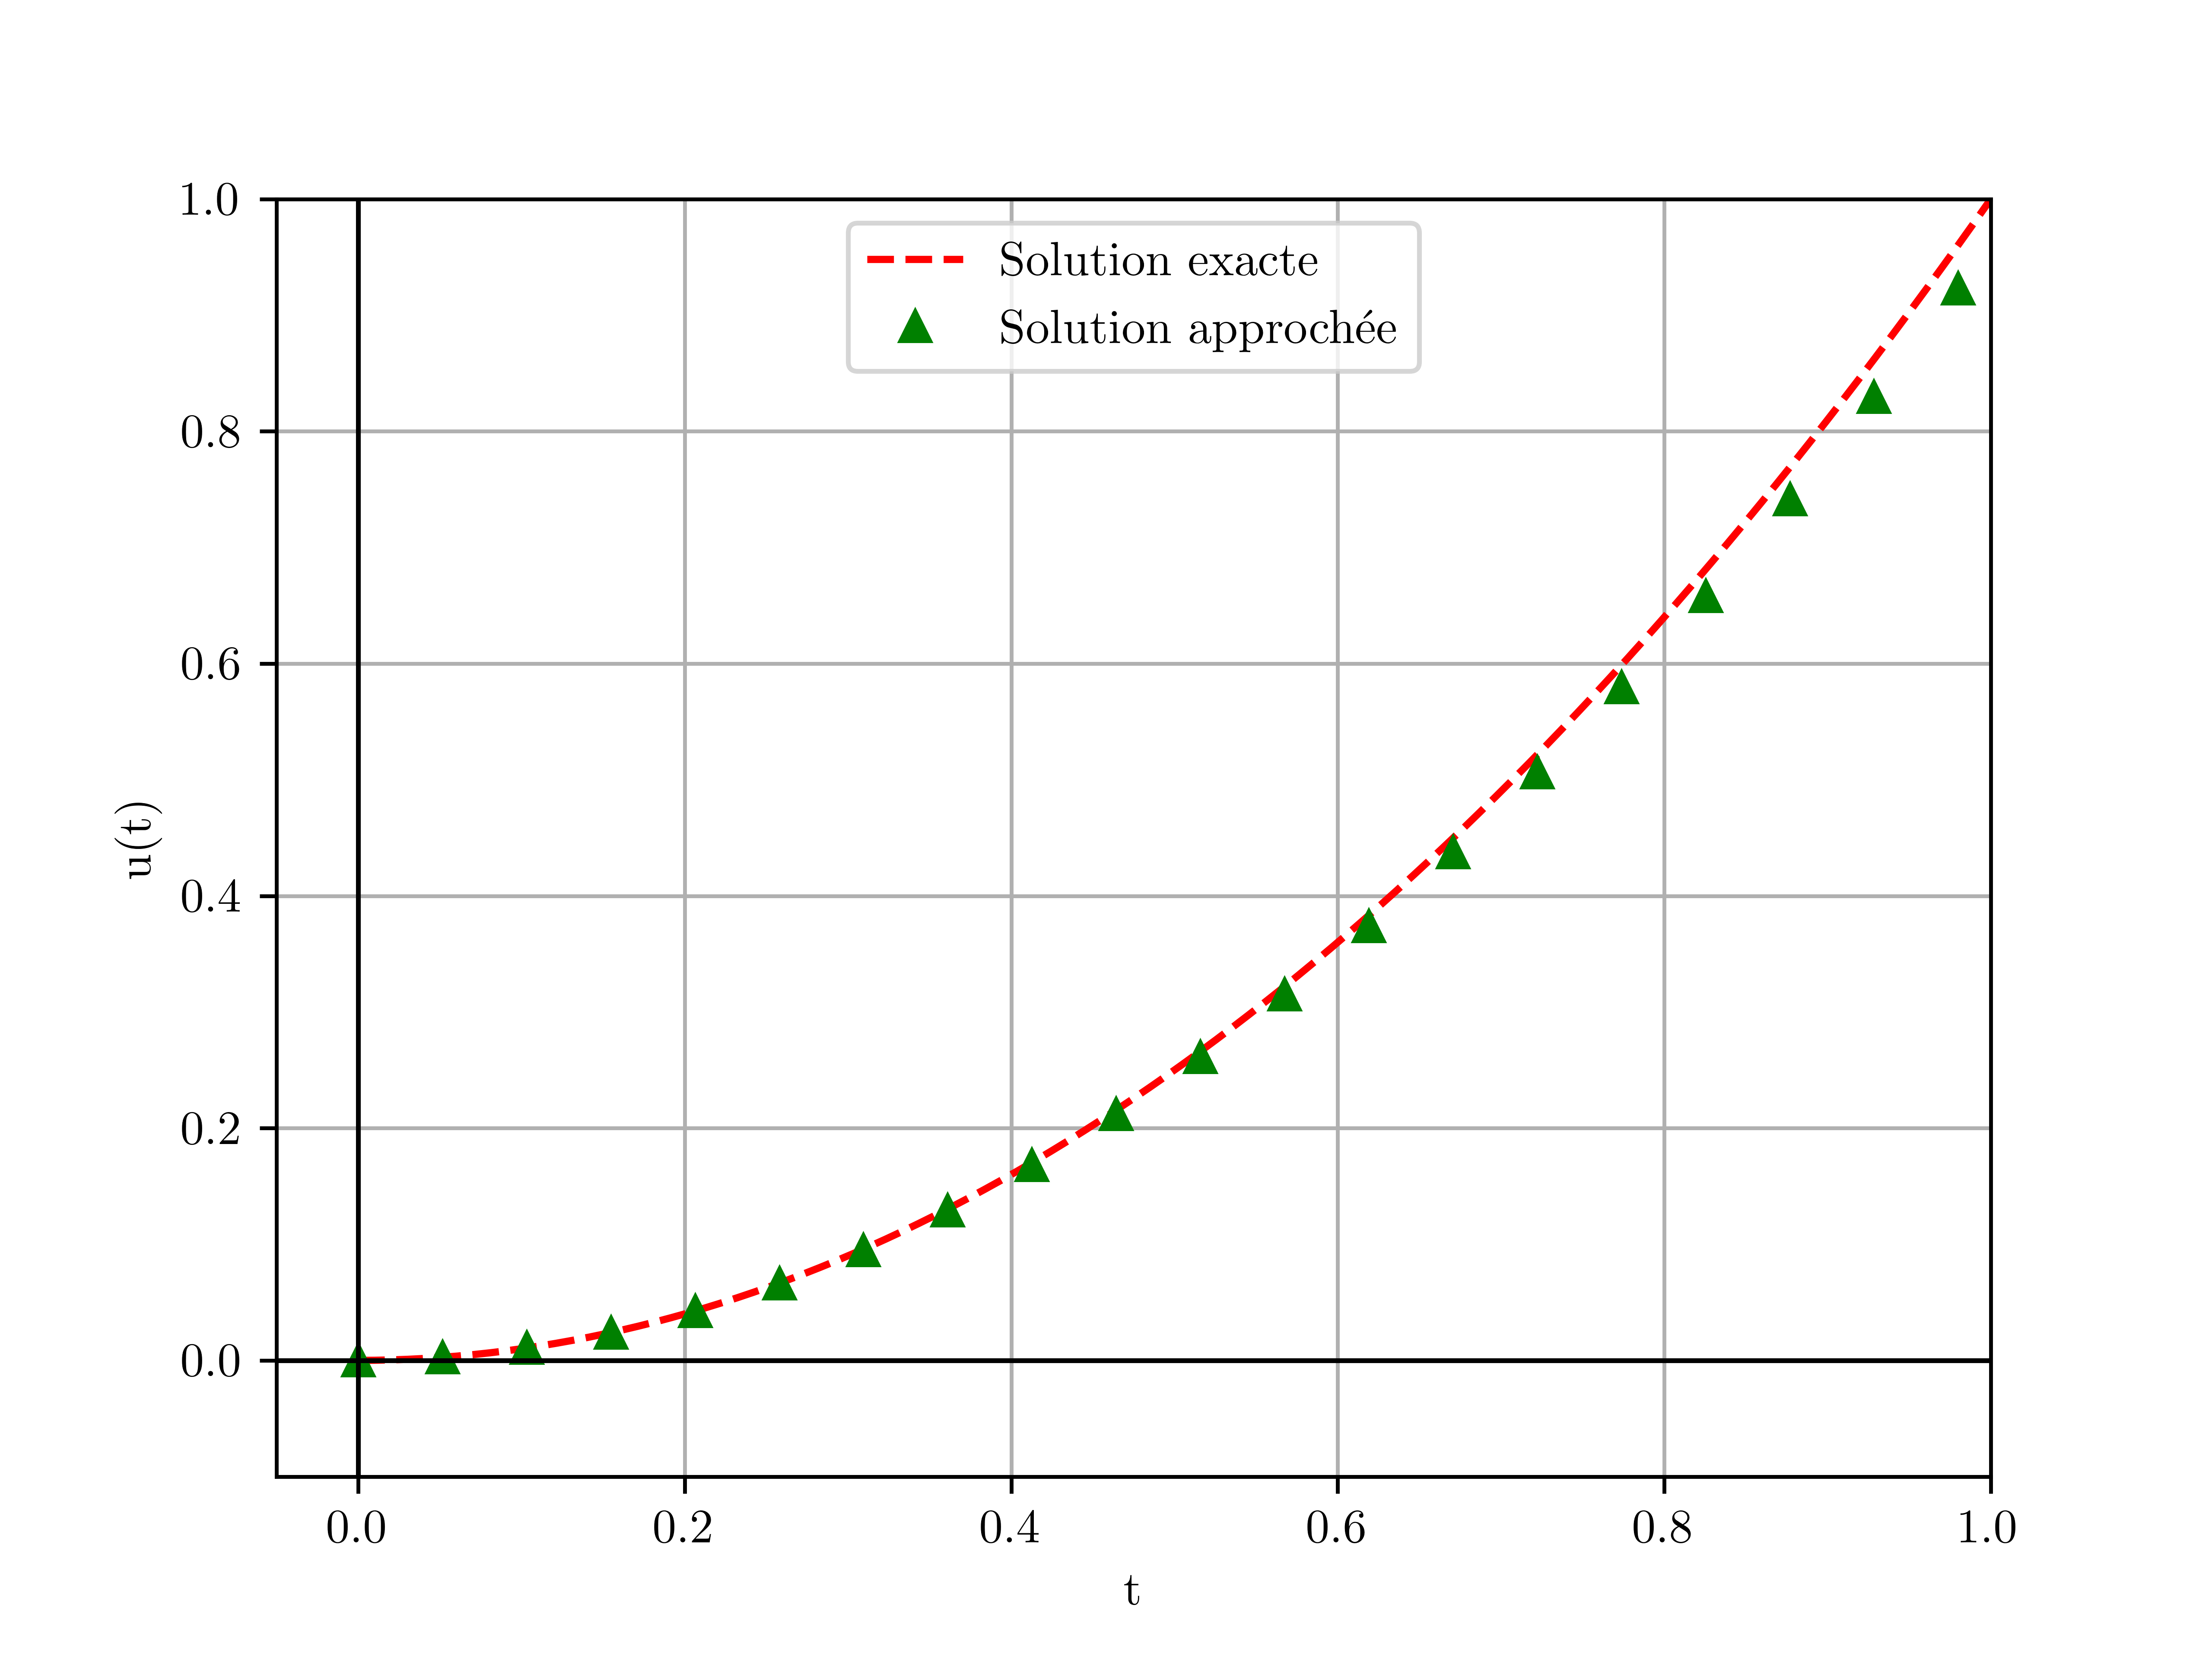
\includegraphics[scale = 0.7]{IMAGES/plot (3).png}
    \caption{Comparaison entre la solution exacte et la solution approchée en utilisant la MPH.}
\end{figure}

\subsubsection*{Exemple 2}
Maintenant, considérons la deuxième équation différentielle factionnaire linéaire suivante :
\begin{equation}\label{ex:EDF_2}
    \begin{cases}
        D^{\alpha} x(t) +x(t) = 1\\
        x(0)=0\\
        x'(t) =0
    \end{cases}
\end{equation}
où la solution exacte est donnée par:
\begin{equation}
    x(t)=t^{1,1} E_{1,1. 2,1} (-t^{1,1})
\end{equation}
Selon la méthode de perturbation d'Homotopie, nous pouvons construire l'homotopie suivante:
\begin{equation} \label{eq:HPM_EDF2}
    D_{\alpha} x(t) +p\left[x(t)-1\right]=0
\end{equation}
La solution de \ref{ex:EDF_1} peut être exprimée comme suit :
\begin{equation}\label{sol:EDF_2}
    x=x_0 + px_1 + p^2x_2 ... = \sum _{i=0}^{\infty} p^i x_i
\end{equation}
Substituons l'équation \ref{sol:EDF_2} dans l'équation \ref{eq:HPM_EDF2} et identifions les termes de même puissance de $p$, il vient :
\begin{align*}
    \sum_{i=0}^{\infty} D^{\alpha} p^{(i)}x_i(t) = p\left(1-\sum_{i=0}^{\infty} p^{i}x_i (t) \right)
\end{align*}
\begin{align}\label{eq:p_2}
\begin{cases}
    & p^0 : D^{\alpha}x_0(t)=0, \\
    & p^1 : D^{\alpha}x_1(t) = 1 -x_0(t),\\
    & p^2 : D^{\alpha} x_2(t) = -x_1(t),\\
    & p^3 : D^{\alpha} x_3(t) = -x_2(t),\\
    &     . \\
    &     .\\
    &     .\\
\end{cases}
\end{align}
Appliquent l'opérateur $I^{\alpha}$ sur les deux cotés de d'équations \ref{eq:p_2} et on utilisons les propriétés de L'intégrale fractionnaire de Riemann-Liouville d'ordre $\alpha \geq 0$, on obtient \begin{align*}
    I^\alpha D^{\alpha} x_0(t) &= x_0(t)-\sum_{i=0}^1 \frac{x^{(i)}(0) t^i}{i!},\\
    &= x_0(t)-x(0)\frac{t^0}{0!}-x'(0)\frac{t^1}{1!}\\
    &= x_0(t) = 0
\end{align*}
\begin{align*}
    I^{\alpha} D^{\alpha}x_1(t) &= x_1(t) - \sum_{i=0}^1 \frac{x^{(i)}(0) t^i}{i!} = x_1(t)\\
    x_1(t) &= I^{\alpha} \left[1-x_0(t)\right]\\
    &= I^{\alpha} [1]\\
    &= \frac{t^{\alpha}}{\Gamma(\alpha +1)}.
\end{align*}
\begin{align*}
    I^{\alpha} D^{\alpha}x_2(t) &= x_2(t) - \sum_{i=0}^1 \frac{x^{(i)}(0) t^i}{i!} = x_2(t)\\
    x_2(t) &= - I^{\alpha} \left[\frac{t^{\alpha}}{\Gamma(\alpha +1)}\right]\\
    &= -\frac{1}{\Gamma(\alpha +1)} \frac{\Gamma(\alpha+1)}{\Gamma(2\alpha +1)} t^{2\alpha}\\
    & = - \frac{t^{2\alpha}}{\Gamma(2\alpha+1)}.
\end{align*}
\begin{align*}
     I^{\alpha} D^{\alpha}x_3(t) &= x_3(t) - \sum_{i=0}^1 \frac{x^{(i)}(0) t^i}{i!} = x_3(t)\\
    x_3(t) &= - I^{\alpha} \left[ - \frac{t^{2\alpha}}{\Gamma(2\alpha+1)} \right]\\
    &= \frac{1}{\Gamma(2\alpha +1)} \frac{\Gamma(2\alpha+1)}{\Gamma(2\alpha +1 + \alpha)} t^{2\alpha + \alpha}\\
    & = \frac{t^{3\alpha}}{\Gamma(3\alpha+1)}.
\end{align*}
Nous obtenons :
\begin{align*}
    & x_0(t) = 0\\
    & x_1(t) = \frac{t^{\alpha}}{\Gamma(\alpha +1)}\\
    & x_2(t) = -\frac{t^{2\alpha}}{\Gamma(2\alpha +1)}\\
    & x_3(t) = \frac{t^{3\alpha}}{\Gamma(3\alpha+1)}\\
    & . \\
    & . \\
\end{align*}
Donc la solution de l'équation \ref{ex:EDF_2} est donnée par:
\begin{align*}
        x(t) &= x_0(t) + px_1(t) + p^2x_2(t) + p^3x_3(t)+...\\
        & = 0 + \frac{t^{\alpha}}{\Gamma(\alpha +1)} -\frac{t^{2\alpha}}{\Gamma(2\alpha +1)} + \frac{t^{3\alpha}}{\Gamma(3\alpha+1)} +...\\
        &= \sum_{K=1}^{\infty}(-1)^{k+1}\frac{t^{k\alpha}}{\Gamma(k\alpha +1)}
\end{align*}
si $\alpha = 1,1$
\begin{align*}
    x(t) &= \frac{t^{1,1}}{\Gamma(2,1)} - \frac{t^{2,2}}{\Gamma(3,2)} +\frac{t^{3,3}}{\Gamma(4,3)} - \frac{t^{4,4}}{\Gamma(5,4)}+...\\
    &= \frac{t^{1,1}}{0.95135} - \frac{t^{2,2}}{0,95135} +\frac{t^{3,3}}{0.95135} - \frac{t^{4,4}}{0.95135}+...\\
    & = 0.95557t^{1,1} - 0.41255t^{2,2} + 0.11293t^{3,3}- 0.02242 t^{4,4} + ...
\end{align*}
De même, en utilisant les solutions exactes extraites de l'article \cite{Numerical_sol} et en déterminant les solutions approchées grâce à la méthode de perturbation d'homotopie, calculées à l'aide de Wolfram Alpha., nous obtenons le tableau \ref{tab:2}. Ce tableau présente les valeurs numériques des solutions exactes, des solutions approchées, ainsi que l'erreur entre ces deux types de solutions. En outre, une comparaison des deux résultats est illustrée dans la figure ci-dessous.
\begin{figure}[H]
    \centering
    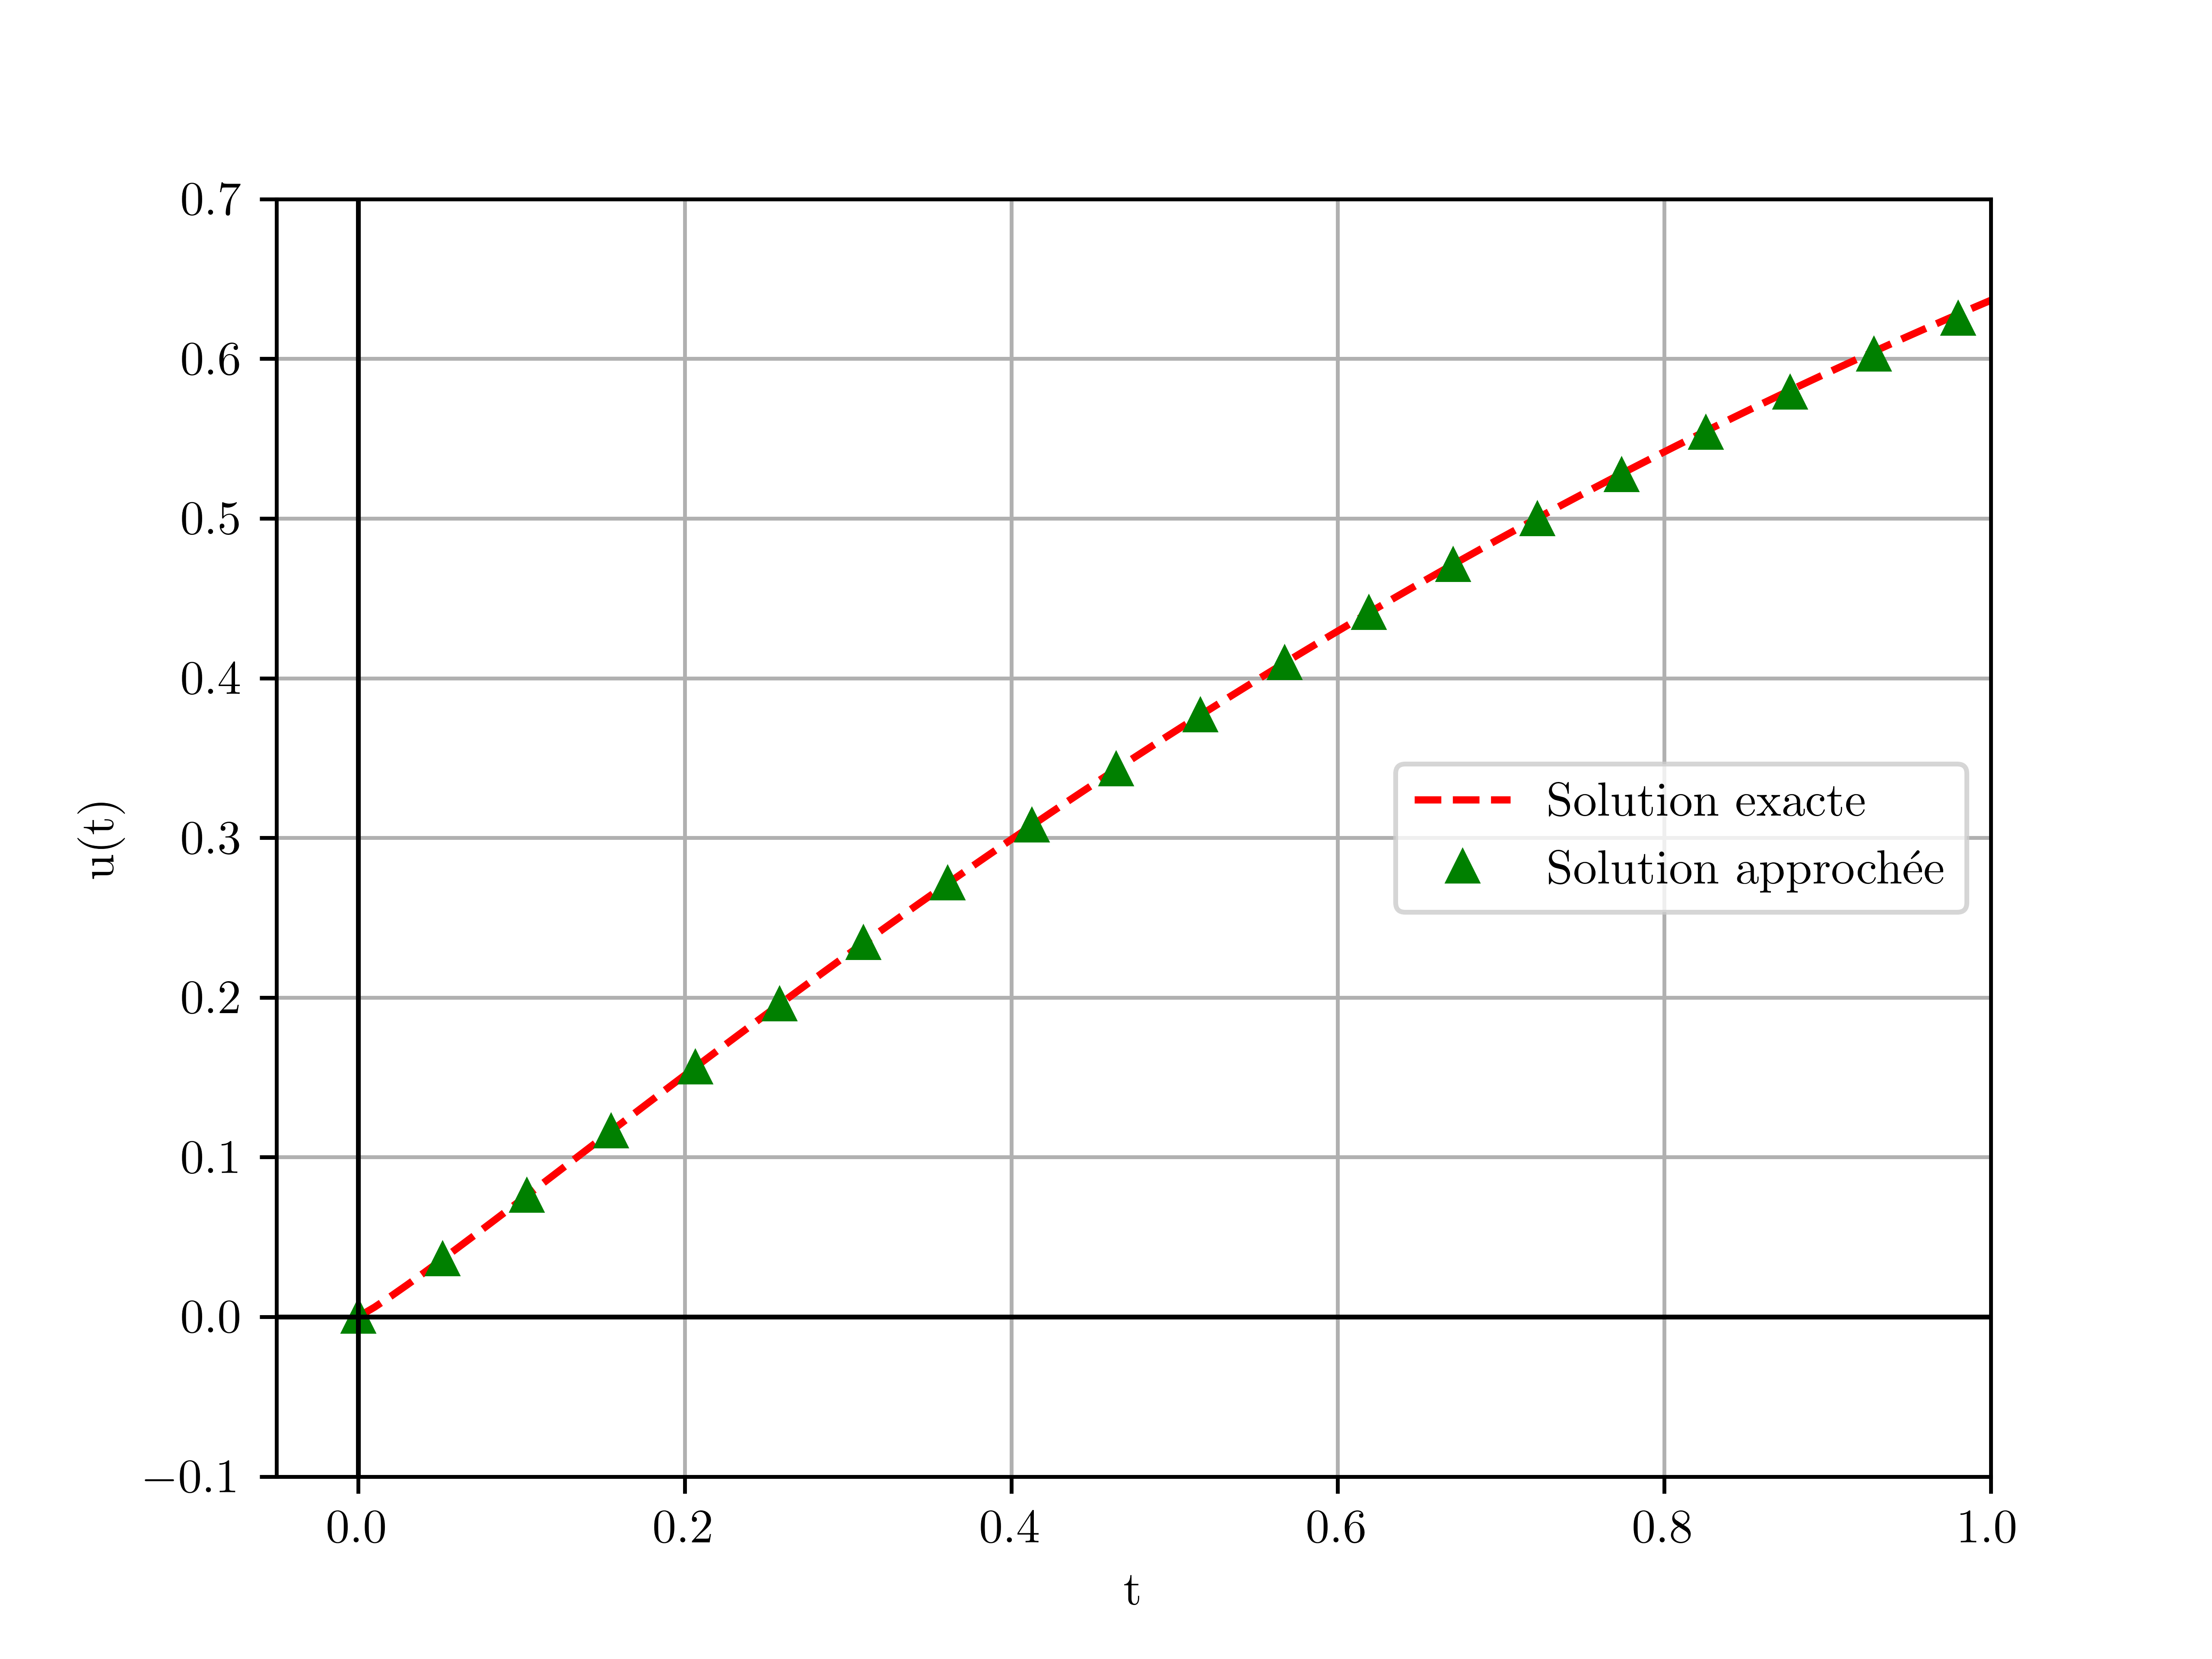
\includegraphics[scale = 0.7]{IMAGES/plot (6).png}
    \caption{Comparaison entre la solution exacte et la solution approchée en utilisant la MPH.}
\end{figure}